\section{hash functions}

\begin{frame}
	%\frametitle{Was sie tun}
	\frametitle{what they do}
	%Eigenschaften
	Propertys:
	\begin{columns}
	\column{6cm}
		\begin{itemize}
		%	\item Surjektiv \begin{small}(Eindeutige Abbildung)\end{small}
		%	\item Kollisionsfrei
		%	\item Lawineneffekt
			\item surjective \begin{small}(unambiguous projection)\end{small}
			\item collision free
			\item good averlancheffect
		\end{itemize}
	\column{6cm}
		\begin{center}
			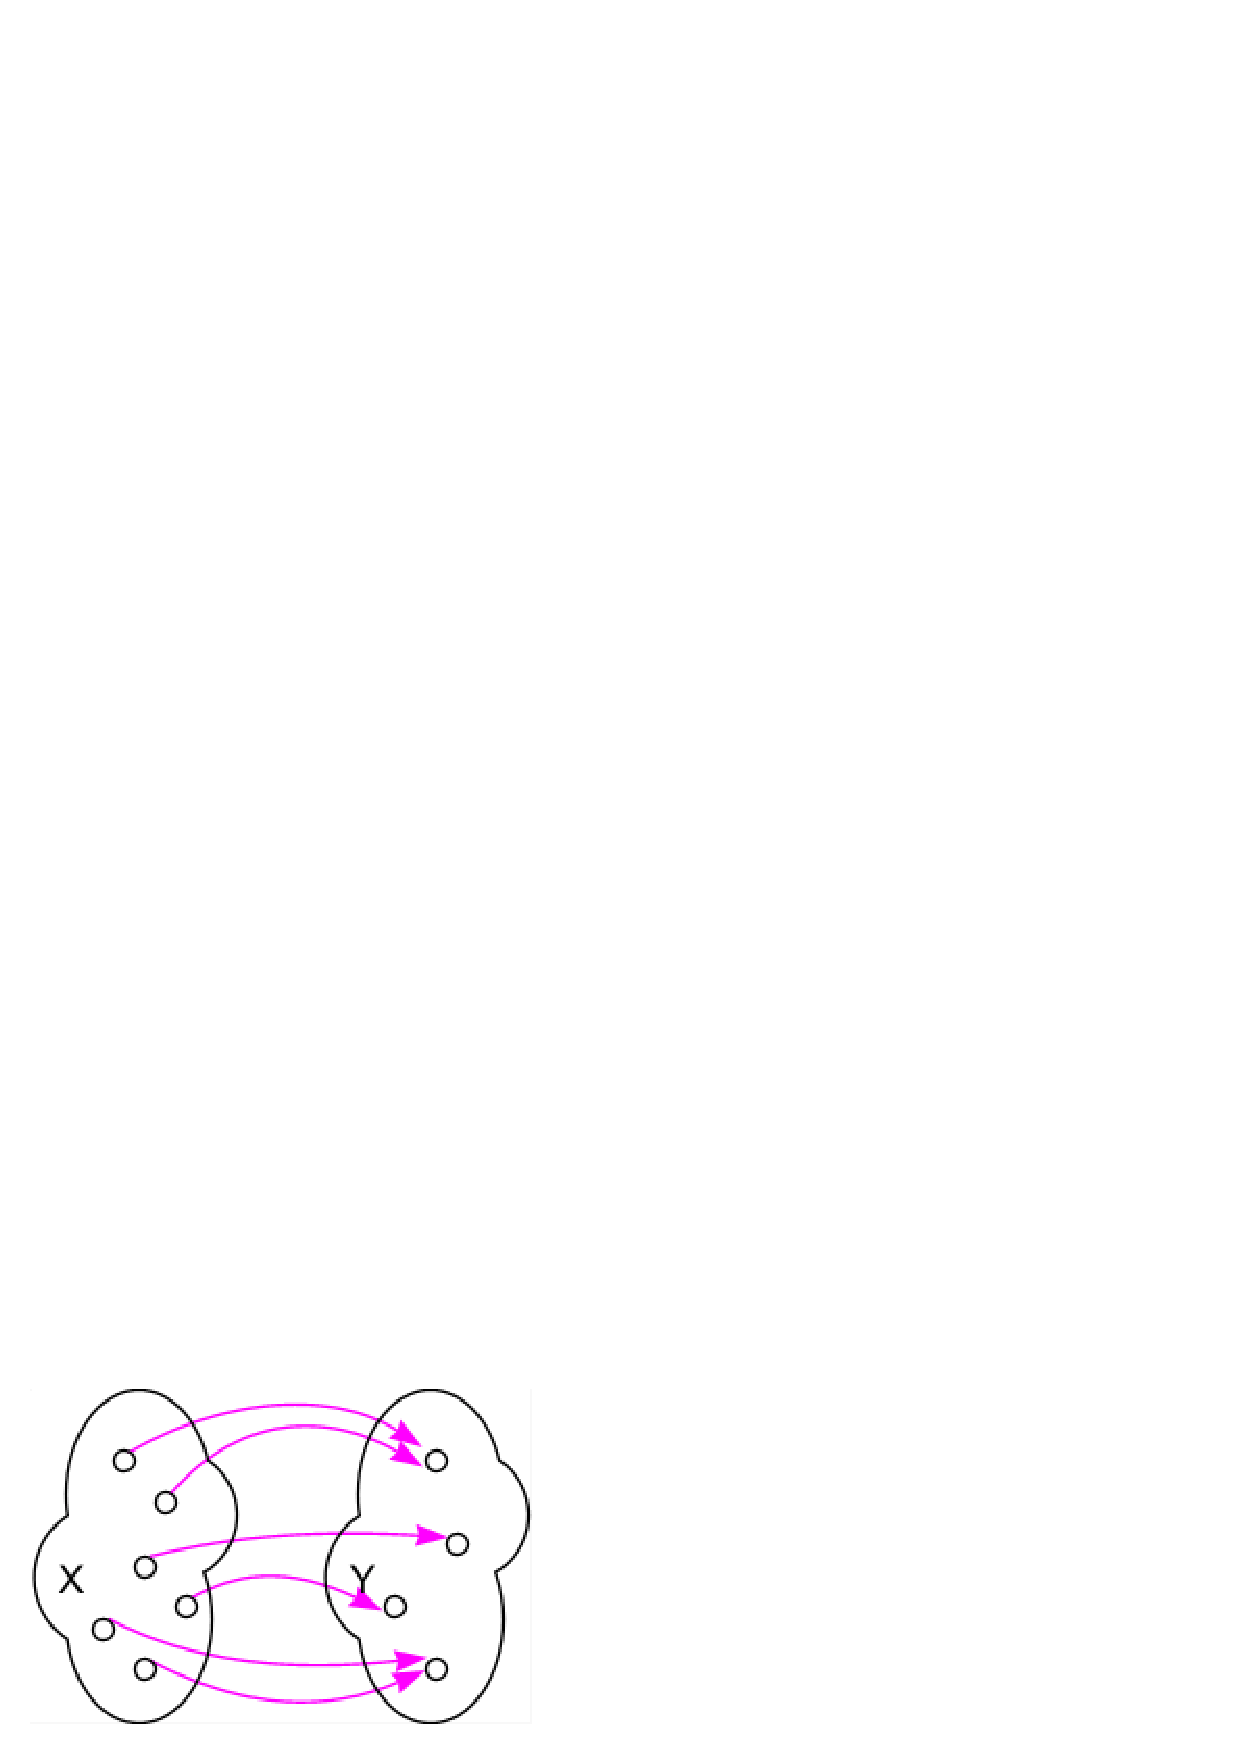
\includegraphics[width=4.8cm,height=3.2cm]{surjektiv}
		\end{center}
	\end{columns}
\end{frame}

\begin{frame}
	\frametitle{example of usage}
	Alice and Bob want to make a decission, where there normaly would flip a coin for.
	But they can not meet and have only a halfduplex communication channel (ex. a telephoneline).
	\begin{enumerate}
		\item Alice generates a random bitstring $m$ of sufficient length (ex. 512 bit) and keeps it secret
		\item Alice sends Bob the hash value $h(m)$ of $m$
		\item Bob ''guesse'' the value of the least significant (or other well defined) bit and sends his guess to Alice
		\item Alice now sends $m$ to Bob
		\item Bob validates that the recieved hash matches the hash of the recieved bitstring $m$
	\end{enumerate}	
\end{frame}

%\begin{frame}
%\frametitle{Warum?}
%	\begin{columns}
%	\column{6cm}
%		\begin{itemize}
%			\item One-way Eigenschaft
%			\item Sinnvoll f"ur gro"se Nachrichten
%		\end{itemize}
%	\column{6cm}
%		\begin{center}
%			
\includegraphics[width=4cm,height=6cm]{oneway}
%		\end{center}
%	\end{columns}
%\end{frame}


\begin{frame}
\frametitle{Wie?}
	Signieren mit gemeinsamen Schl"ussel
	\par
	\begin{center}\large{\texttt{hash ( key | nachricht )}}\end{center}
	\vspace{5mm}
	Speichern von Passw"ortern
	\par
	\begin{center}\large{\texttt{hash ( seed | passwort )}}\end{center}
\end{frame}

\begin{frame}
\frametitle{Angriffe}
	\begin{itemize}
		\item Rainbow Tables (f"ur Passw"orter)
		\item Probieren (z.B. A..z, 0..9)
		\item Reduktion des Problems/Algorithmus
	\end{itemize}
\end{frame}

\begin{frame}
\frametitle{Gegenma"snahmen (1)}
	\large{Immer Salz verwenden!}
\end{frame}

\begin{frame}
\frametitle{Gegenma"snahmen (2)}
	Kaskadieren von Hashfunktionen:
	\par
	\begin{center}\large{\texttt{$hash_1 (msg) \oplus hash_2(msg)$}}\end{center}
	\vspace{5mm}
	\par
	...aber bitte \large{NICHT} so:
	\par
	\begin{center}\large{\texttt{$hash_1 (hash_2(msg))$}}\end{center}
\end{frame}

\end{document}
